\documentclass[12pt, a4paper, oneside]{ctexart}
\usepackage{amsmath, amsthm, amssymb, bm, color, graphicx, geometry, mathrsfs,extarrows, braket, booktabs, array, xcolor, fontspec, appendix, float, subfigure, wrapfig, enumitem, titlesec, bbm}
\usepackage[colorlinks,linkcolor=red,anchorcolor=blue,citecolor=blue,urlcolor=blue,menucolor=black]{hyperref}

%%%% 设置中文字体 %%%%
% fc-list -f "%{family}\n" :lang=zh >d:zhfont.txt 命令查看已有字体
\setCJKmainfont{方正书宋.ttf}[BoldFont = 方正黑体_GBK.ttf, ItalicFont = simkai.ttf, BoldItalicFont = 方正粗楷简体.ttf]
%%%% 设置英文字体 %%%%
\setmainfont{Times New Roman}
\setsansfont{Calibri}
\setmonofont{Consolas}

%%%% 设置代码块 %%%%
% 在vscode中使用minted需要先配置python解释器, Ctrl+Shift+P, 输入Python: Select Interpreter选择安装了Pygments的Python版本. 再在setting.json中xelatex和pdflatex的参数中加入 "--shell-escape", 即可
% TeXworks中配置方法参考: https://blog.csdn.net/RobertChenGuangzhi/article/details/108140093
\usepackage{minted}
\renewcommand{\theFancyVerbLine}{
    \sffamily\textcolor[rgb]{0.5,0.5,0.5}{\scriptsize\arabic{FancyVerbLine}}} % 修改代码前序号大小
% 加入不同语言的代码块
\newmintinline{cpp}{fontsize=\small, linenos, breaklines, frame=lines}
\newminted{cpp}{fontsize=\small, baselinestretch=1, linenos, breaklines, frame=lines}
\newmintedfile{cpp}{fontsize=\small, baselinestretch=1, linenos, breaklines, frame=lines}
\newmintinline{matlab}{fontsize=\small, linenos, breaklines, frame=lines}
\newminted{matlab}{fontsize=\small, baselinestretch=1, mathescape, linenos, breaklines, frame=lines}
\newmintedfile{matlab}{fontsize=\small, baselinestretch=1, linenos, breaklines, frame=lines}
\newmintinline{python}{fontsize=\small, linenos, breaklines, frame=lines, python3}  % 使用\pythoninline{代码}
\newminted{python}{fontsize=\small, baselinestretch=1, linenos, breaklines, frame=lines, python3}  % 使用\begin{pythoncode}代码\end{pythoncode}
\newmintedfile{python}{fontsize=\small, baselinestretch=1, linenos, breaklines, frame=lines, python3}  % 使用\pythonfile{代码地址}

%%%% 设置行间距与页边距 %%%%
\linespread{1.3}
\geometry{left=2.5cm, right=2.5cm, top=2.5cm, bottom=2.5cm}
% \geometry{left=1.84cm,right=1.84cm,top=2.18cm,bottom=2.18cm}  % 更小的页边距

%%%% 定理类环境的定义 %%%%
\newtheorem{example}{例}            % 整体编号
\newtheorem{theorem}{定理}[section] % 定理按section编号
\newtheorem{definition}{定义}
\newtheorem{axiom}{公理}
\newtheorem{property}{性质}
\newtheorem{proposition}{命题}
\newtheorem{lemma}{引理}
\newtheorem{corollary}{推论}
\newtheorem{condition}{条件}
\newtheorem{conclusion}{结论}
\newtheorem{assumption}{假设}
\numberwithin{equation}{section}  % 公式按section编号 (公式右端的小括号)
\newtheorem{algorithm}{算法}

%%%% 自定义环境 %%%%
\newsavebox{\nameinfo}
\newenvironment{myTitle}[1]{
    \begin{center}
    {\zihao{-2}\bf #1\\}
    \zihao{-4}\it
}{\end{center}}  % \begin{myTitle}{标题内容}作者信息\end{myTitle}
\newcounter{problem}  % 问题序号计数器
\newenvironment{problem}[1][]{\stepcounter{problem}\par\noindent\textbf{题目\arabic{problem}. #1}}{\smallskip\par}
\newenvironment{solution}[1][]{\par\noindent\textbf{#1解答. }}{\smallskip\par}  % 可带一个参数表示题号\begin{solution}{题号}
\newenvironment{note}{\par\noindent\textbf{注记. }}{\smallskip\par}
\newenvironment{remark}{\begin{enumerate}[label=\textbf{注\arabic*.}]}{\end{enumerate}}
\BeforeBeginEnvironment{minted}{\vspace{-0.5cm}}  % 缩小minted环境距上文间距
\AfterEndEnvironment{minted}{\vspace{-0.2cm}}  % 缩小minted环境距下文间距

%%%% 自定义段落开头序号,间距 (titlesec) %%%%
% 中文序号:\zhnum{section}, 阿拉伯序号:\arabic
\titleformat{\section}{\Large\bfseries}{第\zhnum{section}章}{1em}{}[]
\titlespacing{\section}{0pt}{1.2ex plus .0ex minus .0ex}{.6ex plus .0ex}
\titlespacing{\subsection}{0pt}{1.2ex plus .0ex minus .0ex}{.6ex plus .0ex}
\titlespacing{\subsubsection}{0pt}{1.2ex plus .0ex minus .0ex}{.6ex plus .0ex}

%%%% 图片相对路径 %%%%
\graphicspath{{figures/}} % 当前目录下的figures文件夹, {../figures/}则是父目录的figures文件夹
\setlength{\abovecaptionskip}{-0.2cm}  % 缩紧图片标题与图片之间的距离
\setlength{\belowcaptionskip}{0pt} 

%%%% 缩小item,enumerate,description两行间间距 %%%%
\setenumerate[1]{itemsep=0pt,partopsep=0pt,parsep=\parskip,topsep=5pt}
\setitemize[1]{itemsep=0pt,partopsep=0pt,parsep=\parskip,topsep=5pt}
\setdescription{itemsep=0pt,partopsep=0pt,parsep=\parskip,topsep=5pt}

%%%% 自定义公式 %%%%
\everymath{\displaystyle} % 默认全部行间公式, 想要变回行内公式使用\textstyle
\DeclareMathOperator*\uplim{\overline{lim}}     % 定义上极限 \uplim_{}
\DeclareMathOperator*\lowlim{\underline{lim}}   % 定义下极限 \lowlim_{}
\DeclareMathOperator*{\argmax}{arg\,max}  % 定义取最大值的参数 \argmax_{}
\DeclareMathOperator*{\argmin}{arg\,min}  % 定义取最小值的参数 \argmin_{}
\let\leq=\leqslant % 简写小于等于\leq (将全部leq变为leqslant)
\let\geq=\geqslant % 简写大于等于\geq (将全部geq变为geqslant)
\DeclareRobustCommand{\rchi}{{\mathpalette\irchi\relax}}
\newcommand{\irchi}[2]{\raisebox{\depth}{$#1\chi$}} % 使用\rchi将\chi居中

%%%% 一些宏定义 %%%%
\def\bd{\boldsymbol}        % 加粗(向量) boldsymbol
\def\disp{\displaystyle}    % 使用行间公式 displaystyle(默认)
\def\tsty{\textstyle}       % 使用行内公式 textstyle
\def\sign{\text{sign}}      % sign function
\def\wtd{\widetilde}        % 宽波浪线 widetilde
\def\R{\mathbb{R}}          % Real number
\def\N{\mathbb{N}}          % Natural number
\def\Z{\mathbb{Z}}          % Integer number
\def\Q{\mathbb{Q}}          % Rational number
\def\C{\mathbb{C}}          % Complex number
\def\K{\mathbb{K}}          % Number Field
\def\P{\mathbb{P}}          % Polynomial
\def\E{\mathbb{E}}          % Expectation
\def\1{\mathbbm{1}}         % Schematic functions
\def\d{\mathrm{d}}          % differential operator
\def\e{\mathrm{e}}          % Euler's number
\def\i{\mathrm{i}}          % imaginary number
\def\P{\mathrm{P}}            % probabilty
\def\re{\mathrm{Re}}        % Real part
\def\im{\mathrm{Im}}        % Imaginary part
\def\res{\mathrm{Res}}      % Residue
\def\ker{\mathrm{Ker}}      % Kernel
\def\vspan{\mathrm{vspan}}  % Span  \span与latex内核代码冲突改为\vspan
\def\L{\mathcal{L}}         % Loss function
\def\O{\mathcal{O}}         % big O notation
\def\wdh{\widehat}          % 宽帽子 widehat
\def\ol{\overline}          % 上横线 overline
\def\ul{\underline}         % 下横线 underline
\def\add{\vspace{1ex}}      % 增加行间距
\def\del{\vspace{-1.5ex}}   % 减少行间距

%%%% 正文开始 %%%%
\begin{document}
\begin{myTitle}{强化学习学习笔记}
    强基数学002\ 吴天阳
\end{myTitle}
\setcounter{section}{1}
\section{多臂赌博机}
\begin{definition}[多臂赌博机]
    k臂赌博机(k-armed Bandits)有一台机器包含$k$种\textbf{动作(Action)}可进行选择,每个动作对应一个概率分布,在做出动作选择后,
    会从对应的概率分布中采样得到对应的\textbf{收益(Reward)},目标是在有限的时间内与赌博机进行交互,并达到最大总收益.

    数学表示:设存在$k$个不同的分布$f_k(\cdot)$,分别对应$k$个动作,总共存在$T$个时刻,在时刻$t$选择的动作记为$A_t$,
    得到的收益(Reward)记为$R_t$,并且$R_t$来自分布$f_{A_t}$,通过在每个时刻与机器进行交互从而最大化$\sum_{t=1}^TR_t$.
\end{definition}

我们将每个动作收益的期望值记为$q_*(a)$,则其满足$q_*(a) := \E[R_t|A_t = a]$,通过不断地和机器进行交互,从而得到$q_*(a)$的估计. 
于是在$t$时刻,我们将$q_*(a)$的估计量记为$Q_t(a)$,称为$a$对应的\textbf{价值(Value)}.

假设我们有$q_*(a)$,并且$q_*(a)$不会随时间发生变换,那么通过贪心的思想,不难得到,每次选择最大收益对应的动作即可最大化全局收益,
但是事实并不如此,其一我们仅有$q_*(a)$的估计量$Q_t(a)$,所以不能保证估计量的准确性;其二,现实场景中的往往是非平稳的(Nonstationary Problem),
也就是指收益的分布会随时间等因素发生变换,而不是保持一个稳定的分布不变. 所以我们的算法不能一味地贪心选择当前最优价值,而是以一定概率探索新的动作,
从而得到可能更优的价值. 具体而言,每次动作的选择会分为\textbf{探索与利用}两种:
\begin{equation*}
    \left\{
        \begin{aligned}
            &\text{1. 利用(Exploitation):贪心操作,选择}\argmax_{a}Q_t(a)\text{作为当前执行的动作.}\\
            &\text{2. 探索(Exploration):以非贪心操作执行动作.}
        \end{aligned}
    \right.
\end{equation*}
强化学习中很重要的一个问题就是如何去平衡探索与利用两种操作.

\subsection{动作-价值方法}
动作-价值方法(Action-value Methods)是指用价值来进行动作的选择. 一种自然的估计价值的方法是用收益的均值:
\begin{equation*}
    Q_t(a) := \frac{\sum_{i=1}^{t-1}R_i\1_{A_i=a}}{\sum_{i=1}^{t-1}\1_{A_i=a}}
\end{equation*}
其中$\1_{A_i=a} = \begin{cases}
    1,&\quad A_i=a,\\
    0,&\quad \text{否则}.
\end{cases}$,下面引入的$\varepsilon$-贪心算法($\varepsilon$-greedy)是一种常用的平衡探索与利用的方法.
\begin{algorithm}[$\varepsilon$-贪心]
该算法以$\varepsilon$的概率在全部动作集合中随机选择(探索),
以$1-\varepsilon$的概率以贪心的方法选择$\argmax_aQ_t(a)$(利用).
\end{algorithm}
\subsubsection{均值估计的增量法}
增量法(Incremental Implementation)是对均值估计的改进,如果直接通过均值公式计算时间复杂度会不断上升,我们考虑通过递推的方式求解$Q_t(a)$,
下面只考虑对于某个特定的动作为$a$,当前时刻之前总共选择了$n$次动作$a$,每次选择所获得的收益为$\{R_1,R_2,\cdots,R_n\}$,则
\begin{equation}\label{eq-average}
\begin{aligned}
    Q_{n+1} =&\ \frac{1}{n}\sum_{i=1}^nR_{i} = \frac{1}{n}\left(R_n + \sum_{i=1}^{n-1}R_i\right) = \frac{1}{n}\left(R_n + (n-1)Q_n\right)\\
    =&\ Q_{n-1}+\frac{1}{n}(R_n - Q_n) = Q_{n-1} + \alpha(t)(R_n - Q_n)
\end{aligned}
\end{equation}
其中$Q_{n+1},R_n$分别表示第$n$次选择动作$a$后动作$a$的价值与收益,$\alpha(t):=1/n$称为\textbf{步长(StepSize)},
有时为常量,有时可随时间发生变换,例如这里与时间成反比关系.
\subsubsection{指数近因估计}
在上述均值估计中,使用的是变换的步长,如果我们将其取为$(0,1)$中的常量$\alpha$,则
\begin{equation}\label{eq-recency}
\begin{aligned}
    Q_{n+1} = Q_n + \alpha(R_n - Q_n) =&\ \alpha R_n + \alpha(1-\alpha)R_{n-1}+\cdots+\alpha(1-\alpha)^{n-1}R_1 + (1-\alpha)^n Q_1\\
    =&\ (1-\alpha)^nQ_1 + \sum_{k=1}^n \alpha(1-\alpha)^{n-k}R_k
\end{aligned}
\end{equation}
由于系数之和满足
\begin{equation*}
    (1-\alpha)^n+\alpha\sum_{k=1}^n(1-\alpha)^{n-k} = (1-\alpha)^n + \alpha\sum_{k=1}^n(1-\alpha)^k = (1-\alpha)^n+\frac{1-(1-\alpha)^n}{\alpha}\alpha = 1
\end{equation*}
则(\ref{eq-recency})式是对$\{Q_1,R_1,\cdots,R_n\}$的一种加权平均,且随时间差的增大,权重以指数形式递减,越靠近当前时刻的权重越大,
于是这种方法也称为\textbf{指数近因加权平均(exponential recency-weighted average)}.

在随机逼近论中有以下定理,常用于判断估计量是否能依概率收敛到真实值上:
\begin{theorem}
    设$\alpha_n$为某个动作第$n$步的步长,若$\{\alpha_n\}$满足
    \begin{equation*}
        \sum_{n=1}^\infty \alpha_n = \infty\quad\text{且}\quad\sum_{n=1}^\infty \alpha_n^2<\infty
    \end{equation*}
    即$\{\alpha_n\}\in \ell^2\backslash\ell^1$时,$Q_n$能以概率$1$收敛到真实值$q_*$,即$\forall \varepsilon > 0$,有
    \begin{equation*}
        \lim_{n\to\infty}\P(|Q_n-q_*|<\varepsilon) = 1
    \end{equation*}
\end{theorem}
上述定理中,$\{\alpha_n\}\notin \ell^1$说明步长需要足够大,以克服初始条件或随机波动,$\{\alpha_n\}\in\ell^2$是保证收敛性.

注意到:当$\alpha_n=1/n$时,$Q_n$收敛,这也是大数定律所保证的;但当$\alpha\in(0,1)$为常值时,上述定理失效,
说明估计永远无法完全收敛,而是随最近得到的收益变换而变换,但在非平稳环境中这种方法的效果比收敛的效果更好.

\begin{example}[练习2.5]
    设计实验来证实使用均值估计方法取解决非平稳问题的困难,使用一个10臂赌博机,其中所有的$q_*(a)$初始时均相等,
    然后进行随机游走,每一步所有的$q_*(a)$都加上一个服从$N(0,0.01^2)$的增量,分别使用均值估计方法和
    指数近因加权估计方法且步长$\alpha=0.1$进行决策,采用$\varepsilon$-贪心进行动作选择,且总步数为$T=10000$.
\end{example}
\begin{solution}
    如图\ref{fig-averge_recency}所示进行了2000次不同的多臂赌博机实验的平均结果,从中非常容易得出,指数近因估计在处理多臂赌博机问题上
    比均值估计要好.
\end{solution}
\begin{figure}[htbp]
    \centering
    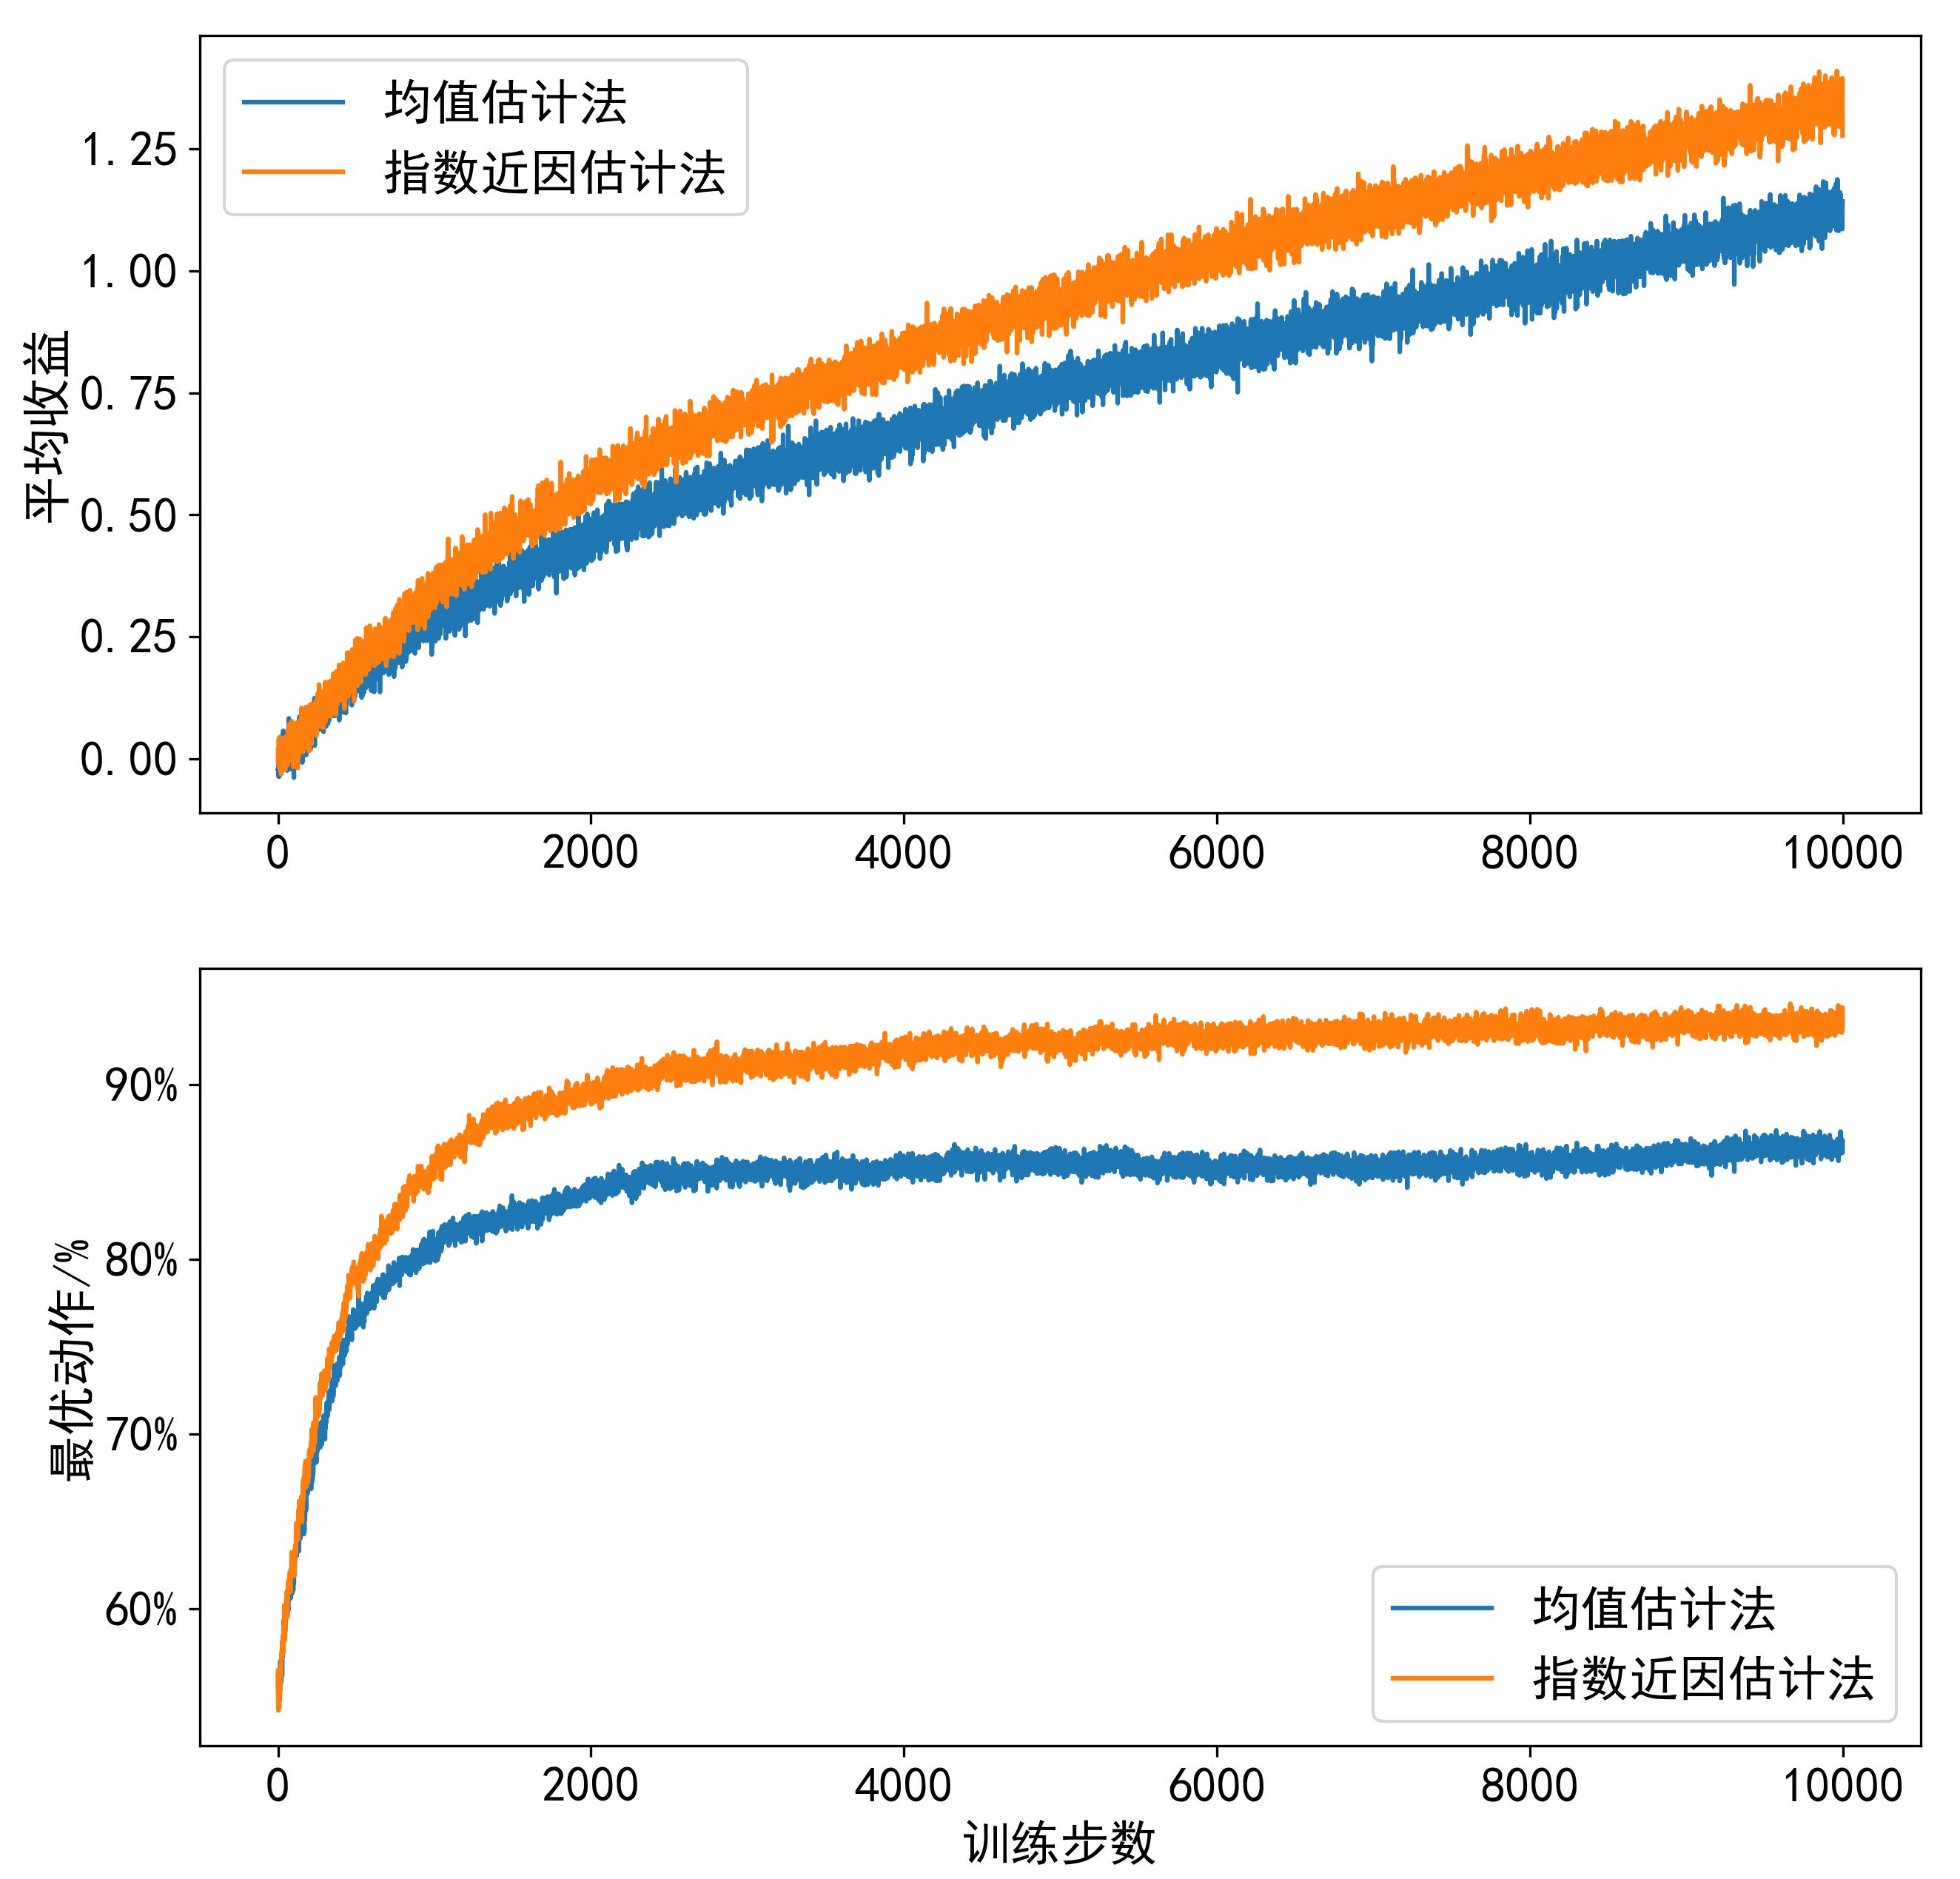
\includegraphics[scale=0.13]{../figures/033页练习2.5.png}
    \caption{非稳定问题中均值法与指数近因法的对比}
    \label{fig-averge_recency}
\end{figure}
\end{document}
